\section{Zielsetzung}
\label{sec:Zielsetzung}

In diesem Versuch soll das Elastizitätsmodul verschiedener Metallen mit verschiedenen Formen bestimmt werden und die gemessenen Daten sollen mit Literaturwerten verglichen werden. 

\section{Theorie}
\label{sec:Theorie}

\subsection{Allgemein}
Durch das Einwirken von Kräften auf einen Körper kann es zur Verformung des Körpers kommen. In der Physik wird von Spannungskräften gesprochen, wenn diese auf den Flächeninhalt bezogen sind. Die Spannung wird in zwei anderen Kräften gegliedert: die Normalspannung $\sigma$, die senkrecht zur Oberfläche steht und die Tangentialspannung, die zur Oberfläche parallele zeigt. Es entsteht somit eine relative Längenänderung, die im Fall, dass sie klein genug ist, ein Zusammenhang zwischen der Normalspannung $\sigma$ und der Deformation zeigt. Dieser Zusammenhang wird in der Physik als Hookesches Gesetz bezeichnet und ist gegeben als: 
\begin{equation}
\label{eqn: Hooke}
\sigma = E \cdot \frac{\Delta L}{L}.
\end{equation}
Dabei bezeichnet der Proportionalitätsfaktor $E$ den Elastizitätsmodul, der in der Werkstofftechnik eine wichtige Größe darstellt.
In diesem Versuch wird der Elastizitätsmodul unter Anwendung der speziellen Deformation, der Biegung, bestimmt. 

\subsection{Einseitige Einspannung}
Wirkt eine Kraft $F$ auf einen einseitigen eingespannten stabförmigen Probekörper, so entsteht eine Durchbiegung $D(x)$. Dieser ist in der Abbildung \ref{fig:einseitig} zu sehen. 
\begin{figure}[h!]
	\centering
	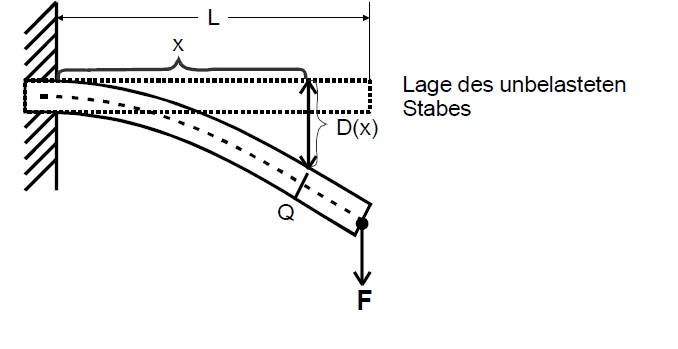
\includegraphics[width=0.7\linewidth]{../../einseitig}
	\caption{Durchbiegung eines einseitig eingespannten Stabes, \cite[2]{anleitung103}.}
	\label{fig:einseitig}
\end{figure}
Es lässt sich in der Abbildung \ref{fig:einseitig} erkennen, dass entgegen der Kraft $F$, noch die Zugspannung in der oberen Schicht und die Druckspannung in der unteren Schicht wirken, die entgegengesetzt gleich sind, so dass ein Gleichgewicht entsteht:
\begin{equation}
\label{eqn: Gleichgew}
M_\text{F} = M_{\sigma}
\end{equation}
Diese bewirken ein Drehmoment $M_{\sigma}$, welches sich über die Integration über den Querschnitt $Q$ errechnen lässt:
\begin{equation}
\label{eqn: Msigma}
M_{\sigma} = \int\limits_Q y \cdot \sigma(y) dq
\end{equation}
wobei $y$ der Abstand zur neutralen Faser darstellt. Der neutrale Faser ist der Bereich, wo keine Spannungen auftreten.
Anhand des Kräftepaares kann eine Drehmomentgleichung aufgestellt werden, um die Funktion $D(x)$ zu bestimmen. Dabei ist $D(x)$ die Durchbiegung eines Stabes zwischen belastetem und unbelastetem Zustand. 
Der äußere Drehmoment $M_\text{F}$ auf das Flächenelement $Q$ lässt sich berechnen wie folgendes:
\begin{equation}
M_\text{F} = F(L-x)
\end{equation}
wobei $L$ die Länge der Stabes und $x$ der Abstand des Messpunktes zum Anfang des Stabes sind.
Es wird in die Gleichung \ref{eqn: Gleichgew} eingesetzt und es ergibt sich nun: 
\begin{equation}
\label{eqn:Gleichg}
\int\limits_Q y \cdot \sigma(y) dq = F(L-x).
\end{equation}
Mit ein paar Überlegungen aus der Differentialgeometrie wird die Funktion $D(x)$ hergeleitet. In die Gleichung \ref{eqn:Gleichg} wird das Hookesche Gesetz \ref{eqn: Hooke} für $\sigma(y)$ verwendet und somit folgt:
\begin{align*}
\sigma(y) &= Ey \frac{d^2 D}{dx^2} \\
\Longleftrightarrow E \frac{d^2 D}{dx^2} \int y^2 dq &= F(L-x) 
\end{align*}
mit
\begin{equation}
\label{eqn: flächenträgheitsmoment}
I = \int\limits_Q y^2 dq
\end{equation}
wobei $I$ das Flächenträgheitsmoment ist, welches berechnet werden kann. Nach Integration folgt die Gleichung für die Funktion $D(x)$:
\begin{equation}
D(x) = \frac{F}{2 E I} \cdot (Lx^2 - \frac{x^3}{3})
\end{equation}
für ($0 \leq x \leq L$).

\subsection{Beidseitige Einspannung}
Nun wird der Stab jetzt beidseitig eingespannt. In der Mitte wirkt die Kraft $F$ (siehe Abbildung \ref{fig:beidseitig})  und der Stab lässt sich in zwei Bereiche unterteilen:
\begin{align}
	\text{I}. 0 \leq x \leq \frac{L}{2} \\
	\text{II}. \frac{L}{2} \leq x \leq L.
\end{align}
Es gilt also in diesem Fall für das Drehmoment im ersten Bereich:
\begin{equation*}
M_\text{F1} = -\frac{F}{2} \cdot x
\end{equation*}
Und für den zweiten Bereich:
\begin{equation*}
M_\text{F2} = -\frac{F}{2} \cdot (L-x)
\end{equation*}

Die Berechnungen für die Funktion $D(x)$ folgen analog zum vorherigen Kapitel. Mit ein paar Überlegungen aus der Differentialgeometrie sowie Integrationen, folgt für die beiden Bereiche folgendes:
\begin{align}
D(x) &= \frac{F}{48EI} \cdot (3L^2x - 4x^3) \\
D(x) &= \frac{F}{48EI} \cdot (4x^3 - 12Lx^2 + 9L^2x - L^3).
\end{align}

\begin{figure}[h!]
	\centering
	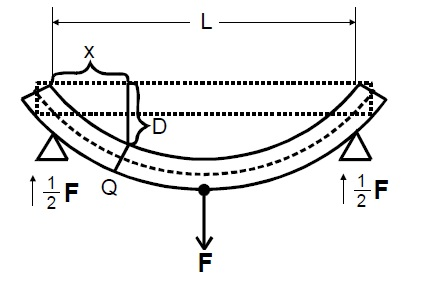
\includegraphics[width=0.7\linewidth]{../../beidseitig}
	\caption{Durchbiegung eines beidseitig eingespannten Stabes, \cite[5]{anleitung103}.}
	\label{fig:beidseitig}
\end{figure}